%
%  $Description: Author guidelines and sample document in LaTeX 2.09$
%
%  $Author: yoonki $
%  $Date: 2009/09/09 18:00:00 $
%  $Revision: 1.4 $
%

\documentclass{sig-alternate}
%\documentclass{acm_proc_article-sp}

\input{macros}
%-- Begin patch area for accents in 'Author Block' area - may be needed by some authors / but not all
\DeclareFixedFont{\auacc}{OT1}{phv}{m}{n}{12}   % Needed for "Author Block" accents - Patch by Gerry 3/21/07
\DeclareFixedFont{\afacc}{OT1}{phv}{m}{n}{10}   % Needed for "Author Block" accents in the affiliation/address line - Patch by Gerry 3/21/07
%--
\begin{document}

\title{Deep Root-Cause Performance Analysis: Integration and Navigation from a Load Testing Tool}

\author{
Yoonki Song\hspace*{0.3in}Tao Xie\\
       \affaddr{Department of Computer Science}\\
       \affaddr{North Carolina State University, Raleigh, USA}\\
       \textit{\email{\{ysong2, txie\}@ncsu.edu}}
}

%-------------------------------------------------------------------------
\maketitle
%\thispagestyle{fancy}

\begin{abstract}
Code Search Engines (CSE) can serve as powerful resources of open
source code, as they can search in billions of lines of open source
code available on the web. The strength of CSEs can be used for
several tasks like searching relevant code samples, identifying
hotspots, and finding bugs. However, the major limitations in using
CSEs for these tasks are that the returned samples are too many and
they are often partial. Our framework addresses the preceding
limitations and thereby helps in using CSEs for these tasks. We
showed the effectiveness of our framework with two tools developed
based on our framework.

\Comment{CSEs are often used by programmers to search for relevant
code samples from publicly accessible source code. However, CSEs are not quite
helpful in practice because the number of returned samples are too many and
the desired code sample is often not available among the first several results.
Apart from using CSEs for searching relevant code samples, CSEs can also be used
for several other applications like identifying framework hotspots and finding bugs
in software. Exploiting CSEs for these applications requires analysis of
the code samples returned by CSEs. This analysis is non-trivial because the code samples
returned by CSEs are often partial.\Comment{, as CSEs retrieve
only source files with usages of the given query instead of entire projects.}
In this paper, we propose an extensible framework that addresses the preceding limitations
and thereby helps in exploiting CSEs for several applications that can help improve the
productivity of programmers. Our framework performs static analysis over code samples gathered from a CSE by
using several heuristics and transforms those samples into graph representations that can be directly
used for other applications. }
\end{abstract}
              % abstract
\section{Introduction}

\label{sec:introduction}

Access control is one of the most fundamental and widely used
security mechanisms. It controls which principals (users, processes,
etc.) have access to which resources in a system. To better manage
access control, systems often explicitly specify access control
policies using policy languages such as XACML~\cite{oasis05:xacml}
and Ponder \cite{damianou01:ponder}. Whenever a principal requests
access to a resource, that request is passed to a software component
called a Policy Decision Point (PDP). PDP evaluates the request
against access control policies, and grants or denies the request
accordingly.

The specification of access control policies is often a challenging
problem. It is common that a system's security is compromised due to
the misconfiguration of access control policies instead of the
failure of cryptographic primitives or protocols. This problem
becomes increasingly severe as software systems become more and more
complex, and are deployed to manage a large amount of sensitive
information and resources that are organized into sophisticated
structures.

Formal verification is an important means to ensuring the correct
specification of access control
policies\Comment{~\cite{jajodia97:logical, sandhu99:arbac}}.
Recently, several tools have been developed to verify XACML access
control policies against user-specified
properties~\cite{hughes04:automated,fisler05:verification,zhang05:evaluating}.
However, it is often beyond the capabilities of these tools to
verify complex access control policies in large-scale information
systems. Furthermore, user-specified properties are often not
available~\cite{fisler05:verification}.

Like in software development, errors in access control policies may
also be discovered through testing. In fact, once access control
policies are specified, they are often tested with some access
requests so that security officers may manually check the PDP's
responses against expected ones~\cite{anderson02:xacml}. However,
current policy testing practice tends to be ad hoc. Although there
exist various coverage criteria~\cite{zhu97:software} for software
programs, there are no criteria or good heuristics to guide
systematic generation of high-quality policy test suites. With an ad
hoc policy testing, it is questionable that high confidence could be
gained on the correctness of access control policies.

This paper presents a first step toward systematic policy testing.
We propose the concept of \Intro{policy coverage} to measure the
quality of policy test suites, which are sets of request-response
pairs. Intuitively, the more policy rules (as well as their
components such as subjects, resources, and conditions) are involved
when evaluating a test suite, the more likely it is to discover
errors in access control policies. We have developed a
coverage-measurement tool to measure the coverage of XACML policies
achieved by a set of access requests. We have also developed a
request-generation tool that randomly generates policy test suites
for a given set of policies.

Although the randomly generated test suites can achieve high policy
coverage, and are effective in detecting a variety of policy
specification errors, it may potentially include a huge number of
requests, which makes it difficult to efficiently inspect and verify
the correctness of responses from the PDP. To mitigate this problem,
we further propose a request reduction technique to significantly
reduce the size of a test suite while maintaining its policy
coverage.

Previous experiments~\cite{rothermel98:empirical} showed that test
reduction based on program code coverage can severely compromise the
fault-detection capabilities of the original test suite. To evaluate
the impact of the proposed request reduction technique on the
quality of policy testing, we conduct an experiment on a set of real
policies with mutation testing~\cite{demillo78:hints}, which is a
specific form of fault injection that consists of creating faulty
versions of a policy by making small syntactic changes. In the
experiment, we compare the fault-detection capabilities of the
reduced set and original set of requests. Our experimental results
show that our coverage-based request reduction technique can
substantially reduce the size of generated requests but incur only
relatively low loss in fault detection capabilities. We also conduct
a study that measures the policy coverage of an XACML conformance
test suite as well as a conference reviewing system's policy. Our
results show that the measurement of policy coverage can effectively
identify uncovered parts of policies. Such results can be used to
guide the development of further test cases, significantly improving
the quality of policy testing.

\Comment{ This paper makes the following main contributions:
\begin{itemize}
\item We propose the concept of policy coverage based on
a general access control model. We further instantiate this
concept in the context of XACML, a widely used and standardized
meta policy language
for expressing domain-specific access control requirements.

\item We develop a coverage-measurement tool for automatically
measuring the coverage for XACML policies achieved by a given set
of requests.

\item We develop a request-generation tool for randomly generating
requests for XACML policies and a request-reduction tool for
greedily selecting a minimal set of requests for achieving the
same policy coverage as the original set of requests.

\item We develop initial mutation operators for XACML policies to
conduct mutation testing. We conduct an experiment on a set of
real policies to compare the effectiveness of the minimal set of
requests with the original set of requests in terms of fault
detection. We also conduct a study on policy coverage of existing
manually generated requests.

\end{itemize}
}

The rest of the paper is organized as follows. Section
\ref{sec:xacml} presents background information on XACML, a widely
used and standardized meta policy language for expressing
domain-specific access control requirements.
Section~\ref{sec:model} proposes the concept of policy testing and
policy coverage based on a general access control model. In
Section~\ref{sec:coverage}, we instantiate the concept of policy
coverage in the context of XACML. We also present the design of a
coverage measurement tool. Sections~\ref{sec:reqgen}
and~\ref{sec:reqreduce} describe the request-generation tool and
our request reduction technique, respectively.
Section~\ref{sec:mutation} presents a set of initial mutation
operators developed for policies. Section~\ref{sec:experiment}
presents the experiment conducted to assess request reduction and
its effect on fault detection capabilities.
Section~\ref{sec:experimentalresults} illustrates the study of
measuring the policy coverage achieved by manually generated
requests. Section~\ref{sec:related} discusses related work and
Section~\ref{sec:conclusion} concludes the paper with future
directions.

















\sloppy
          % 1. Introduction
\section{Approach}
\label{sec:approach}
\begin{figure}[t]
\centering
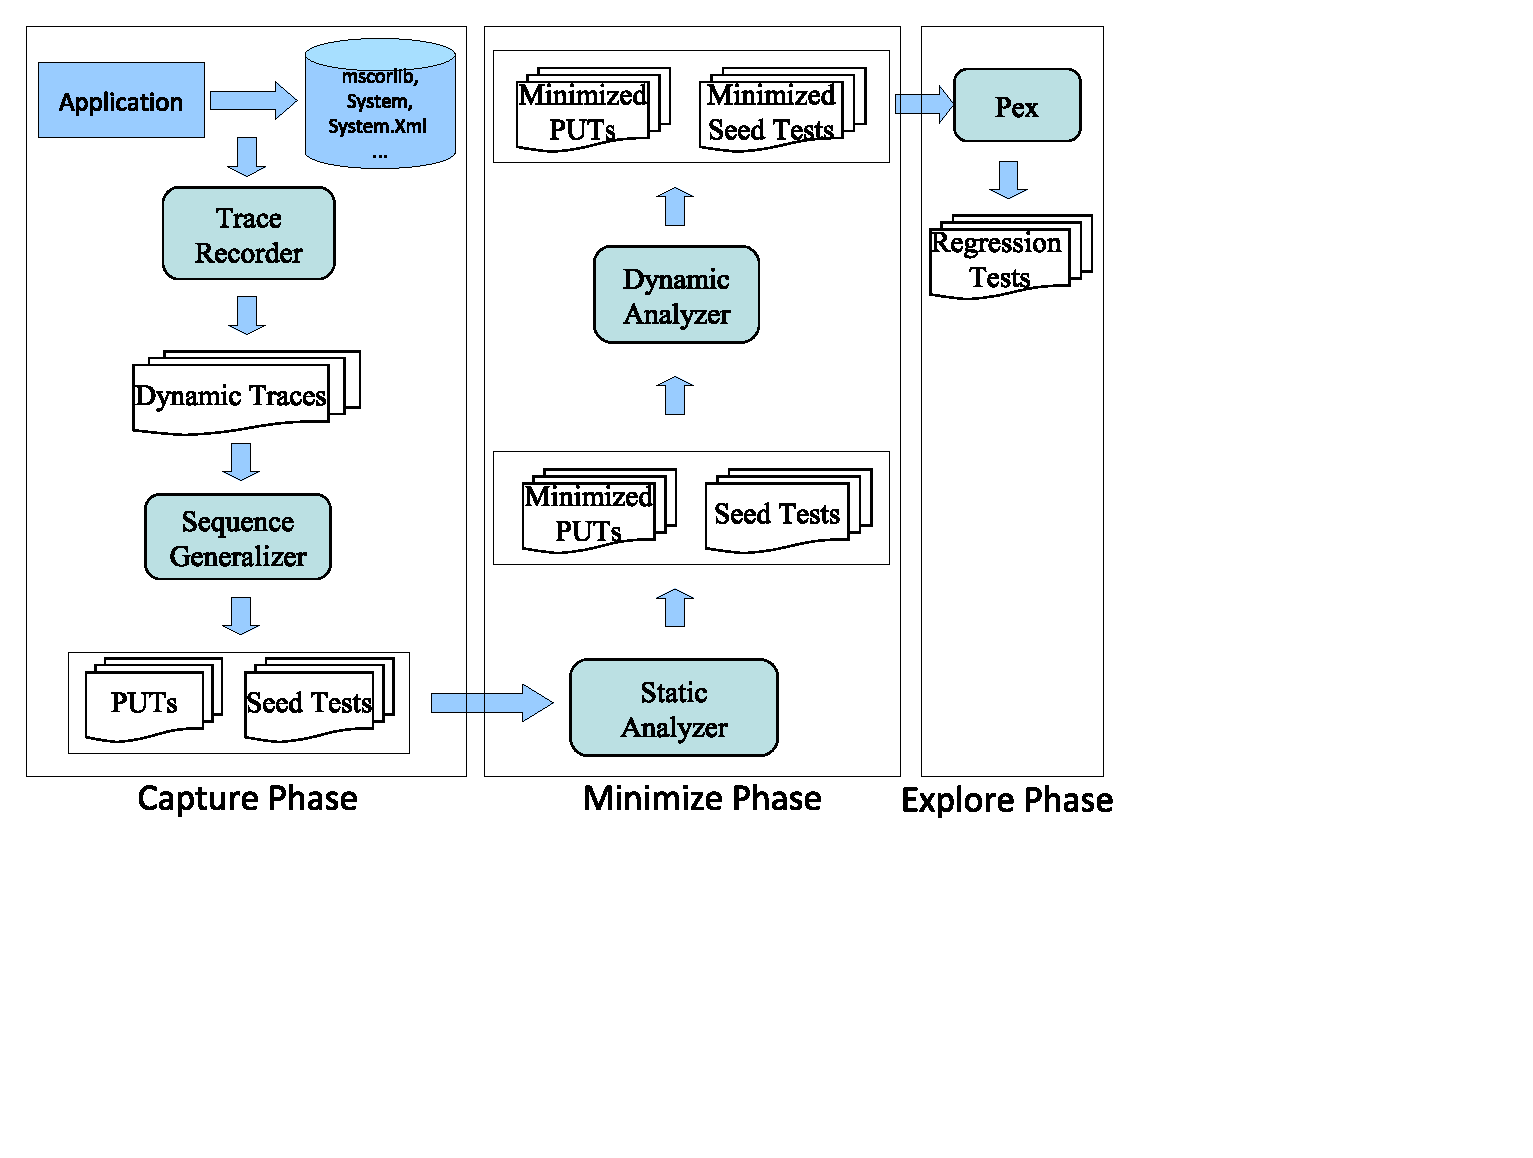
\includegraphics[scale=1,clip]{figure/approach.eps}\vspace*{-3ex}
 \caption{Overview of TeMaAPI}\vspace*{-4ex}
 \label{fig:approach}
\end{figure}
Given a migration tool between Java and C\#, TeMaAPI generates various test cases to reveal different behaviors of the tool's API mapping relations.
Figure~\ref{fig:approach} shows the overview of TeMaAPI.


%-------------------------------------------------------------------
\subsection{Generating client code}
\label{sec:approach:generating}
Given a migration tool, TeMaAPI first extracts its validate mapping relations of APIs. It is challenging to extract such mapping relations directly from a migration tool for two factors: (1) different migration tools may follow different styles to describe API mapping relations. For example, as shown in Section~\ref{sec:introduction}, the API mapping relations of Java2CSharp are described in its mapping files, but the API mapping relations of sharpen are hard-coded in its source files. (2) commercial migration tools typically hide their API mapping relations in binary files. Due to the two factors, TeMaAPI does not extract API mapping relations directly from a migration tool, but chooses to analyze translated code of a migration tool. We choose to use migration tools to translate simple client code instead of existing projects for two considerations: (1) Existing projects typically use quite a small set of APIs, so many API mapping relations may be not covered; (2) a single method of an existing project may use multiple APIs, so it may be difficult to analyze which APIs are not mapped. For the preceding consideration, TeMaAPI chooses to generate client code instead of using existing client code.

TeMaAPI relies on the reflection technique~\cite{maes1987concepts} provided by both Java and C\# to generate client code for translation.

\textbf{Static fields.} Given a public static field \CodeIn{f} of a class \CodeIn{C} whose type is \CodeIn{T}, TeMaAPI generates a getter as follows:
\begin{CodeOut}%\vspace*{-2ex}
\begin{alltt}
 public T TestGet|f.name||no|()\{ return C.f; \}
\end{alltt}
\end{CodeOut}

If \CodeIn{f} is not a constant, TeMaAPI generates a setter as follows:
\begin{CodeOut}%\vspace*{-2ex}
\begin{alltt}
 public void TestSet|f.name||no|(T v)\{ C.f = v; \}
\end{alltt}
\end{CodeOut}

\textbf{Non-static fields.} Given a public non-static field \CodeIn{f} of a class \CodeIn{C} whose type is \CodeIn{T}, TeMaAPI generates a getter for each constructor \CodeIn{C(T1\ p1,\ldots, Tn\ pn)} of \CodeIn{C} as follows:
\begin{CodeOut}%\vspace*{-2ex}
\begin{alltt}
 public T TestGet|f.name||no|(T1\ c1,\ldots, Tn\ cn)\{
    C obj = new C(c1,\ldots, cn);
    return obj.f; \}
\end{alltt}
\end{CodeOut}

If \CodeIn{f} is not a constant, TeMaAPI generates a setter as follows:
\begin{CodeOut}%\vspace*{-2ex}
\begin{alltt}
 public void TestSet|f.name||no|(T1\ c1,\ldots, Tn\ cn)\{
   C obj = new C(c1,\ldots, cn);
   obj.f = v; \}
\end{alltt}
\end{CodeOut}

In the preceding code, ``\CodeIn{|f.name|}'' denotes the name of \CodeIn{f}, and ``\CodeIn{|no|}'' denotes the corresponding number of generated client-code method.

\textbf{Static methods.} Given a public static method \CodeIn{m(T1\ p1,\ldots,Tn\ pn)} of a class \CodeIn{C} whose return type is \CodeIn{Tm}, TeMaAPI generates a client-code method as follows:
\begin{CodeOut}%\vspace*{-2ex}
\begin{alltt}
 public Tm Test|m.name||no|(T1\ m1,\ldots, Tn\ mn)\{
   return C.m(m1,\ldots, mn); \}
\end{alltt}
\end{CodeOut}

\textbf{Non-static methods.} Given a public non-static method \CodeIn{m(T1\ p1,\ldots,Tn\ pn)} of a class \CodeIn{C} whose return type is \CodeIn{Tm}, TeMaAPI generates a client-code method for each constructor \CodeIn{C(Tv\ pv,\ldots, Tt\ pt)} of \CodeIn{C} as follows:
\begin{CodeOut}%\vspace*{-2ex}
\begin{alltt}
 public Tm Test|m.name||no|(T1\ m1,\ldots, Tn\ mn,
                            Tv cv, \ldots, Tt ct)\{
   C obj = new C(cv,\ldots, ct);
   return obj.m(m1,\ldots, mn); \}
\end{alltt}
\end{CodeOut}

In the preceding code, ``\CodeIn{|m.name|}'' denotes the name of \CodeIn{m(T1\ p1,\ldots,Tn\ pn)}.

TeMaAPI ignores generic methods for simplicity, and organizes all generated client code methods by the corresponding class $C$. For a migration tool that translates from Java to C\#, TeMaAPI generates client code in Java as shown by the solid line of Figure~\ref{fig:approach}, and for a migration tool that translates from C\# to Java, TeMaAPI generates client code in C\# as shown by the dotted line of Figure~\ref{fig:approach}. When TeMaAPI generates client code in C\#, it ignores \CodeIn{unsafe} and \CodeIn{delegate} methods and methods whose parameters are marked as \CodeIn{our} or \CodeIn{ref}. Java does not have corresponding keywords, so there are typically no mapped methods in Java for these C\# methods. After TeMaAPI generate client-code methods, we translate them using a migration tool under experiments.


%-----------------------------------------------------------------
\subsection{Analyzing Generated Methods}
\label{sec:approach:analyzing}
Translated code typically contain many compilation errors since a migration tool typically cannot cover mapping relations of all APIs. TeMaAPI then analyzes translated code for validate API mapping relations of the migration tool. To achieve this, TeMaAPI first remove all translated methods with compilation errors. For translated methods in Java, TeMaAPI implements a Eclipse plug-in that uses on Eclipse JDT compiler\footnote{\url{http://www.eclipse.org/jdt/}} for the list of compilation errors. For translated methods in C\#, TeMaAPI implements a Visual Studio.Net add-in to retrieve the list of compilation errors from the error-list view of Visual Studio.Net. Both Eclipse JDT compiler and Visual Studio.Net cannot list all methods with compilation errors in a single build. After each iteration of removing methods, TeMaAPI re-build these methods until it removes all methods with compilation errors.

After methods with compilation errors are removed, TeMaAPI compares generated code with translated code for the validate API mapping relations of a migration tool. Based on translated code and validate API mapping, TeMaAPI removes generated methods whose corresponding translated methods have compilation errors. We refer to those removing client-code methods as safe methods.

%-----------------------------------------------------------
\subsection{Finding Different Behaviors}
\label{sec:approach:behavior}
In the final step, TeMaAPI generates test cases to detect different behaviors of API mapping relations. An alternative approach is to use existing test cases in two languages. For example, lucene\footnote{\url{http://lucene.apache.org}} has both a Java version and a C\# version. It is feasible to use these test cases to reveal some different behaviors, but such test cases typically cover only a small set of APIs. Some test suites such as Java Compatibility Kit (JCK)\footnote{\url{http://jck.dev.java.net}} cover most APIs of a language. However, translating such a test suite from one language into another language may introduce many compilation errors and defects. A test method may use many APIs, so even if the API under test can be translated correctly, the test method cannot be translated correctly since other APIs are not mapped. As a result, we choose to translating existing test suites as a supplement of our approach.

\subsubsection{Generating Test Cases}
\label{sec:approach:behavior:generating}
For each safe method in Java, we use Randoop~\cite{pacheco2007feedback} to generate its test cases. For each safe method in C\#, we use Pex~\cite{tillmann2008pex} to generate its test cases. TeMaAPI then executes generated test cases, and records the inputs, the output, and the thrown exception of each test case as a file.

Based on the file, TeMaAPI generates Junit\footnote{\url{http://www.junit.org/}} or Nunit\footnote{\url{http://www.nunit.org/}} test cases to ensure each mapped API produce the same output give the same inputs. For example, Pex generates a test case whose input is \CodeIn{m0 = false} for the \CodeIn{TestvalueOf57} method in C\# as shown in Section~\ref{sec:example}, and after executing the output of the test case is ``False''. Based on the input and the output of this test case, TeMaAPI generates a Junit test case as follows:

\begin{CodeOut}%\vspace*{-2ex}
\begin{alltt}
 @Test
 public void testvalueOf64zhh0()\{
   sketch.Test_java_lang_String obj =
                       new sketch.Test_java_lang_String();
   boolean m0 = false;
   Assert.assertEquals("False", obj.testvalueOf64(m0));\}
\end{alltt}
\end{CodeOut}

This Junit test case fails since the preceding \CodeIn{testvalueOf64zhh} method produces ``false'' instead of ``False''. From this failed Junit test case, TeMaAPI detects that the \CodeIn{java.lang.String.valueOf (Object)} method in Java has different behaviors with its mapped C\# methods if inputs are boolean values.

In some cases, executing a test case does not produce outputs but exceptions. For example, Pex also generates a test case whose input is \CodeIn{m0 = null} for the \CodeIn{TestvalueOf57} method in C\# as shown in Section~\ref{sec:example}, after executing it throws \CodeIn{NullReferenceException}. TeMaAPI finds that the \CodeIn{NullPointerException} class in C\# is mapped to the \CodeIn{NullPointerException} class in Java in the validate API mapping relations, and generates a Junit test case based on the preceding mapping relation and input as follows:

\begin{CodeOut}%\vspace*{-2ex}
\begin{alltt}
 @Test
 public void testvalueOf64zhh3()\{
   try\{
     sketch.Test_java_lang_String obj =
                       new sketch.Test_java_lang_String();
     boolean m0 = null;
     obj.testvalueOf64(m0);\}
   \}catch(java.lang.NullPointerException e)\{
       Assert.assertTrue(true);
       return;
   \}
   Assert.assertTrue(false);\}
\end{alltt}
\end{CodeOut}

This Junit test case also fails since given a null input, the preceding \CodeIn{testvalueOf64} method does not throw any exceptions. From this failed Junit test case, TeMaAPI detects that the \CodeIn{java.lang. String.valueOf(Object)} method in Java has different behaviors with its mapped C\# methods if inputs are null pointers.

\subsubsection{Translating Existing Test Cases}
\label{sec:approach:behavior:jck}

Each generated client-code method uses only one fields or methods provided by API libraries, and may lose some complicated behaviors even if test cases satisfy the round-trip criterion. To test those complicated behaviors, we introduce JCK that covers many complicated behaviors of Java APIs. JCK is a test suite provided by Sun to ensure compatibility of Java platforms, and it covers most standard APIs of J2SE. However, JCK implements many internal classes to collect the results of executed test cases. If a migration tool cannot correctly translate one of these classes, all translated test cases may have compilation errors or defects. In addition, JCK is released under read-only source license\footnote{\url{http://tinyurl.com/33x9fo6}}, so many such internal classes are not shipped and it has many compilation errors. To increase the chance of migrating JCK, TeMaAPI first replaces those internal classes with the classes of Junit. For example, one test method for \CodeIn{java.io.File.delete()} in JCK is as follows:

\begin{CodeOut}%\vspace*{-2ex}
\begin{alltt}
  public Status File0037()\{
    String testCaseID = "File0037";
    ...
    FileRT method = new FileRT(testCaseID) \{
     public Status run() \{
       File f = null;
       f = new File(workdir, testCaseID);
       ...
       if (f.delete()) \{ // Try to delete
         if (!f.exists()) \{ // Does it exist?
           return Status.passed("OKAY");
         \}else\{
            return Status.failed(...);
         \}
       else\{
           return Status.failed(...);
       \}
    \}
     return AllPermissionSM.testRun(...);
  \}
\end{alltt}
\end{CodeOut}

After the preceding three steps, TeMaAPI further replaces the statement starts with \CodeIn{FileRT} with the body of the \CodeIn{run} method, and removes the last statement. The translated code is as follows:

\begin{CodeOut}%\vspace*{-2ex}
\begin{alltt}
  public void File0037()\{
    String testCaseID = "File0037";
    ...
    File f = null;
    f = new File(workdir, testCaseID);
    ...
    if (f.delete()) \{ // Try to delete
      if (!f.exists()) \{ // Does it exist?
        Assert.assertTrue(true);
        return;
     \}else\{
        Assert.fail();
        return;
     \}
   else\{
       Assert.fail();
       return;
   \}
  \}
\end{alltt}
\end{CodeOut}

Compared with the original test method in JCK, the translated method does not use the three internal classes: \CodeIn{Status}, \CodeIn{FileRT}, and \CodeIn{AllPermissionSM}. 

After the preceding process, for a migration tool, TeMaAPI further removes methods that use any APIs outside its defined mapping relations. The remaining methods can be translated from Java to other languages since it does not use any APIs outside of the migration tool.


              % 2. Approach

\bibliographystyle{is-abbrv}
%\bibliographystyle{abbrv}
\bibliography{yoonki-references,yoonki}  % sigproc.bib is the name of the Bibliography in this case
\end{document}
